\enlargethispage{25pt}
\fancyhead[RO,RE]{\small\textsf{\textbf{BÀI 1.3}}\quad \textsf{Các hàm số mới từ các hàm số cũ}\quad \textbf{43}}
\fancyhead[LO,LE]{}
\fancyfoot{}
\fancyfoot[C]{\fontsize{6pt}{7.5pt}\selectfont\color{gray} Copyright 2021 Cengage Learning. All Rights Reserved. May not be copied, scanned, or duplicated, in whole or in part. WCN 02-200-203}

\begin{multicols}{2}
\fontsize{7.8pt}{9.6pt}\selectfont
\setlength{\abovedisplayskip}{2pt}
\setlength{\belowdisplayskip}{2pt}

\noindent\textbf{4.} Cho đồ thị của $f$. Hãy vẽ đồ thị của các hàm số sau:
\vspace{3pt}

\noindent
\begin{tabular}{@{}p{0.48\linewidth}p{0.48\linewidth}@{}}
(a) $y = f(x) - 3$ & (b) $y = f(x + 1)$ \\[2pt]
(c) $y = \frac{1}{2}f(x)$ & (d) $y = -f(x)$
\end{tabular}

\begin{center}
\vspace{-2pt}
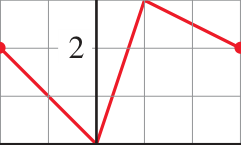
\includegraphics[width=0.55\linewidth]{images/p0078_graph_2.png}
\vspace{-2pt}
\end{center}

\noindent\textbf{5.} Cho đồ thị của $f$. Hãy sử dụng đồ thị đó để vẽ đồ thị của các hàm số sau:
\vspace{3pt}

\noindent
\begin{tabular}{@{}p{0.48\linewidth}p{0.48\linewidth}@{}}
(a) $y = f(2x)$ & (b) $y = f\left(\frac{1}{2}x\right)$ \\[2pt]
(c) $y = f(-x)$ & (d) $y = -f(-x)$
\end{tabular}

\begin{center}
\vspace{-2pt}
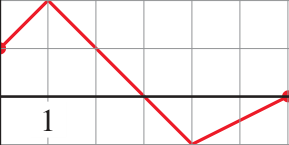
\includegraphics[width=0.55\linewidth]{images/p0078_graph_3.png}
\vspace{-2pt}
\end{center}

\noindent\textbf{\textsf{\color{stewartcyan}6--7}}\quad Cho đồ thị của $y = \sqrt{3x - x^2}$. Hãy sử dụng các phép biến đổi để xác định hàm số có đồ thị như hình vẽ.

\begin{center}
\vspace{-2pt}
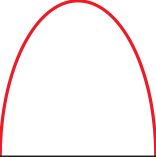
\includegraphics[width=0.55\linewidth]{images/p0078_graph_4.png}
\vspace{-2pt}
\end{center}

\vspace{3pt}
\noindent{\color{stewartcyan!60}\rule{\linewidth}{0.6pt}}
\vspace{3pt}

\noindent\textbf{8.} 
\begin{enumerate}[(a),leftmargin=1.5em,itemsep=1pt,topsep=1pt]
\item Đồ thị của $y = 1 + \sqrt{x}$ có mối liên hệ như thế nào với đồ thị của $y = \sqrt{x}$? Hãy sử dụng câu trả lời của bạn và Hình 4(a) để phác họa đồ thị của $y = 1 + \sqrt{x}$.
\item Đồ thị của $y = 5\sin\pi x$ có mối liên hệ như thế nào với đồ thị của $y = \sin x$? Hãy sử dụng câu trả lời của bạn và Hình 6 để phác họa đồ thị của $y = 5\sin\pi x$.
\end{enumerate}

\vspace{3pt}
\noindent\textbf{\textsf{\color{stewartcyan}9--26}}\quad Hãy vẽ đồ thị hàm số bằng tay, không phải bằng cách lấy từng điểm, mà bắt đầu từ đồ thị của một trong các hàm số chuẩn đã cho trong Bảng 1.2.3, sau đó áp dụng các phép biến đổi thích hợp.
\vspace{3pt}

\noindent
\begin{tabular}{@{}p{0.48\linewidth}p{0.48\linewidth}@{}}
\textbf{9.} $y = 1 + x^2$ & \textbf{10.} $y = (x + 1)^2$ \\[2pt]
\textbf{11.} $y = |x + 2|$ & \textbf{12.} $y = 1 - x^3$
\end{tabular}

\columnbreak

\noindent
\begin{tabular}{@{}p{0.48\linewidth}p{0.48\linewidth}@{}}
\textbf{13.} $y = \dfrac{1}{x} + 2$ & \textbf{14.} $y = -\sqrt{x} - 1$ \\[2pt]
\textbf{15.} $y = \sin 4x$ & \textbf{16.} $y = 1 + \dfrac{1}{x^2}$ \\[2pt]
\textbf{17.} $y = 2 + \sqrt{x + 1}$ & \textbf{18.} $y = -(x - 1)^2 + 3$ \\[2pt]
\textbf{19.} $y = x^2 - 2x + 5$ & \textbf{20.} $y = (x + 1)^3 + 2$ \\[2pt]
\textbf{21.} $y = 2 - |x|$ & \textbf{22.} $y = 2 - 2\cos x$ \\[2pt]
\textbf{23.} $y = 3\sin\frac{1}{2}x + 1$ & \textbf{24.} $y = \frac{1}{4}\tan\left(x - \frac{\pi}{4}\right)$ \\[2pt]
\textbf{25.} $y = |\cos \pi x|$ & \textbf{26.} $y = |\sqrt{x} - 1|$
\end{tabular}

\vspace{3pt}
\noindent{\color{stewartcyan!60}\rule{\linewidth}{0.6pt}}
\vspace{3pt}

\noindent\textbf{27.} Thành phố New Orleans nằm ở vĩ độ $30^\circ\text{B}$. Hãy sử dụng Hình 9 để tìm một hàm số mô hình hóa số giờ có ánh sáng ban ngày tại New Orleans theo thời gian trong năm. Để kiểm tra độ chính xác của mô hình, hãy dùng dữ kiện rằng vào ngày 31 tháng 3, mặt trời mọc lúc 5:51 SA và lặn lúc 6:18 CH tại New Orleans.

\vspace{3pt}
\noindent\textbf{28.} Sao biến quang là ngôi sao có độ sáng luân phiên tăng và giảm. Đối với ngôi sao biến quang dễ quan sát nhất, Delta Cephei, khoảng thời gian giữa các chu kỳ đạt độ sáng cực đại là $5{,}4$ ngày, độ sáng trung bình (hay cấp sao) của ngôi sao là $4{,}0$, và độ sáng của nó biến thiên một lượng $\pm 0{,}35$ cấp sao. Hãy tìm một hàm số mô hình hóa độ sáng của Delta Cephei theo thời gian.

\vspace{3pt}
\noindent\textbf{29.} Một số vùng có thủy triều cao nhất trên thế giới xuất hiện tại vịnh Fundy thuộc bờ biển Đại Tây Dương của Canada. Tại Mũi Hopewell, độ sâu của nước khi triều kiệt là khoảng $2{,}0\text{ m}$ và khi triều cường là khoảng $12{,}0\text{ m}$. Chu kỳ dao động tự nhiên là khoảng 12 giờ và vào một ngày cụ thể, triều cường xảy ra lúc 6:45 SA. Hãy tìm một hàm số chứa hàm cosin để mô hình hóa độ sâu của nước $D(t)$ (tính bằng mét) theo thời gian $t$ (tính bằng giờ sau nửa đêm) vào ngày hôm đó.

\vspace{3pt}
\noindent\textbf{30.} Trong một chu kỳ hô hấp bình thường, thể tích không khí lưu thông vào và ra khỏi phổi là khoảng $500\text{ mL}$. Thể tích dự trữ và thể tích cặn của không khí còn lại trong phổi chiếm khoảng $2000\text{ mL}$ và một chu kỳ hô hấp đơn lẻ của một người bình thường kéo dài khoảng 4 giây. Hãy tìm một mô hình cho tổng thể tích không khí $V(t)$ trong phổi theo thời gian.

\vspace{3pt}
\noindent\textbf{31.} 
\begin{enumerate}[(a),leftmargin=1.5em,itemsep=1pt,topsep=1pt]
\item Đồ thị của $y = f(|x|)$ có mối liên hệ như thế nào với đồ thị của $f$?
\item Hãy phác họa đồ thị của $y = \sin|x|$.
\item Hãy phác họa đồ thị của $y = \sqrt{|x|}$.
\end{enumerate}

\vspace{3pt}
\noindent\textbf{32.} Hãy sử dụng đồ thị đã cho của $f$ để phác họa đồ thị của $y = 1/f(x)$. Những đặc trưng nào của $f$ là quan trọng nhất khi phác họa đồ thị $y = 1/f(x)$? Hãy giải thích cách sử dụng chúng.

\begin{center}
\vspace{-2pt}
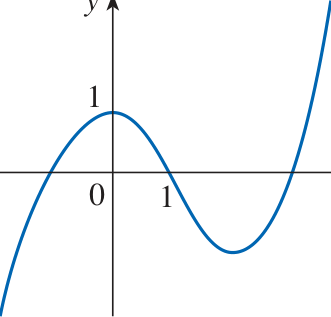
\includegraphics[width=0.48\linewidth]{images/p0078_graph_1.png}
\vspace{-2pt}
\end{center}

\end{multicols}